\documentclass[11pt]{IEEEtran}
% correct bad hyphenation here
%\hyphenation{op-tical net-works semi-conduc-tor}

\usepackage{algorithm, algpseudocode, amsmath, cite, graphicx, multirow, url}

\makeatletter
\newcommand{\removelatexerror}{\let\@latex@error\@gobble}
\makeatother

\renewcommand\thesection{\arabic{section}}
\renewcommand\thesubsection{\thesection.\arabic{subsection}}
\renewcommand\thesubsubsection{\thesubsection.\arabic{subsubsection}}

\renewcommand\thesectiondis{\arabic{section}}
\renewcommand\thesubsectiondis{\thesectiondis.\arabic{subsection}}
\renewcommand\thesubsubsectiondis{\thesubsectiondis.\arabic{subsubsection}}

\begin{document}

\title{Tag Recommendations in StackOverflow}
\author{Logan~Short, Christopher~Wong, and~David~Zeng}% <-this % stops a space
\markboth{CS 224W Final Project, Autumn 2014}{}
\maketitle

\begin{abstract}
Abstract goes here.
\end{abstract}

\section{Introduction}

\IEEEPARstart{I}{n} many community-based information web sites, such as StackOverflow, users contribute content in the form of questions and answers, allowing others to learn through the collaboration and contributions of the community. These web sites often rely upon tags as metadata that assists in the indexing, categorization, and search for particular content with just a few key words. Almost always, users are given the responsibility to choose tags which identify their own content. Tagging, however, can prove to be a confusing process for inexperienced users who may not be familiar with the tags available to them. In addition, general human error or malicious users could lead to improperly tagged posts that disrupt the organization of information on the website.

As such, there is a clear motivation behind implementing stronger and more accurate tag recommendation systems. The most obvious benefit stems from the fact that tags help ensure that website data is properly categorized and thus easily searchable by users. A tag recommendation model can improve tag accuracy and effectiveness in a number of ways. For example, new users would not have to worry as much when choosing appropriate tags for their questions, and so the act of asking questions is an easier experience along with the better tags being chosen. Furthermore, recommending tags decreases the possibility of introducing \textit{tag synonyms} into the tagspace, as is commonly done through human error. Tag synonyms are discussed more in Section 3.

The development of tag recommendation systems for user created content is a relatively new field and most previous work has taken place within the last couple of years. Thus, tag recommending is a field in which the state of the art is still being actively developed, and the most accurate methods for recommending tags have yet to be established. Software information web sites and other such services that are based on user produced content rely on the interactions between users and consequently are governed by an underlying network structure. It is thus probable that network structure could be used to assess user content and obtain accurate tag recommendations. Based on this intuition, the goal of our work is to analyze whether the underlying network structure of software information sites can be used to accurately recommend tags for user produced content and to potentially advance the state of the art in this still developing field.

\section{Prior Work and Motivation}

We first surveyed the recent literature and research in tag recommendation systems to get an idea of what improvements we could make. We discovered two recent papers, published in 2013 and 2014, that detail two algorithms, \textit{TagCombine} and \textit{EnTagRec}, for tag recommendation on sites like StackOverflow. The improvements we can make to these algorithms (Section 2.3), along with recent discussion about community detection in graphs (Section 2.4), give us motivation for a new, improved tag recommendation model.

\subsection{TagCombine Algorithm}

In \cite{1}, Xia et al. propose an automatic tag recommendation algorithm \textit{TagCombine}. There are three components of \textit{TagCombine}, each of which tries to assign the best tags to untagged objects: (1) multi-label ranking component, which predicts tags using a multi-label learning algorithm, (2) similarity based ranking component, which uses similar objects to recommend tags, and (3) tag-term based ranking component, which analyzes the historical affinity of tags to certain words in order to suggest tags. The recommendation algorithm methodically computes various weighted sums of the three components to attempt to find the best overall model. A $recall@k$ score is then calculated for each prediction model from stratified $10$-fold cross validation. (The $recall@k$ metric is discussed more in Section $4$.) The results demonstrate that \textit{TagCombine} performs significantly better than all other cited models.

\subsection{EnTagRec Algorithm}

In \cite{2}, Wang et al. propose a tag recommendation system dubbed \textit{EnTagRec}. The proposed \textit{EnTagRec} computes tag probability scores using two separate methods, Bayesian Inference and Frequentist Inference, and then takes a weighted sum of the probability scores. Bayesian Inference relies on a post’s textual data to compute the probability that a given tag is associated with the post. \textit{EnTagRec} formulates posts into a bag-of-words model and then trains a Labeled Latent Dirichlet Allocation model which is used to compute tag probability scores for a post. The Frequentist Inference approach infers a set of tags after some preprocessing of a post, and then utilizes a network of tags to select additional tags that are similar to the ones in the set. The network of tags is constructed with the tags as nodes and weighted edges between two tags and based on the Jaccard similarity of the posts that contain those tags. Experimental results show that \textit{EnTagRec} performs significantly better than \textit{TagCombine} from \cite{1} on Stack Overflow, Ask Ubuntu, and Ask Different datasets, but yields only comparable results on Freecode datasets.

\subsection{Motivation for NetTagCombine}

In \cite{1}, Xia et al. propose a recommendation system that relates the textual features of posts to tags with reasonably good results. However, one weakness of \textit{TagCombine} is that it fails to look at the network structure of software information sites. Posts on sites like Stack Overflow are ultimately connected to each other through an underlying network structure where users and tags that appear on multiple posts represent connections between said posts. In fact, the main purpose of tags is to group similar posts and create an organized structure that allows for more convenient and logical browsing of posts. Thus, it is not too farfetched to conjecture that knowledge of the network’s structure could be used to enhance a tag recommendation system. In fact, in \cite{2}, Wang et al. use not only textual analysis of posts, but also basic network analysis of the tags.  Although the results of \textit{EnTagRec} outperformed those of \textit{TagCombine}, it is difficult to quantify the improvement directly caused by the network features, as the machine learning models used by the two algorithms are also different. Our proposed algorithm, \textit{NetTagCombine}, will use \textit{TagCombine} as its baseline, instead of \textit{EnTagRec} primarily because \textit{TagCombine} has no network features to begin with. By adding network related components for tag recommendation to \textit{TagCombine}, we can unambiguously quantify the improvement these network features have to offer by directly comparing our results to those of \textit{TagCombine}. Furthermore, the machine learning models used in \textit{TagCombine} are also simpler than those used in \textit{EnTagRec}, making them more tractable to implement in the timeframe we were given.

\subsection{Prior Work in Community Detection}

In \cite{3}, McAuley and Leskovec discuss a method for automatically detecting ``circles'' in networks of users based on similarities in user profiles. This motivated us to consider using community detection in improving tag recommendation. Since tags serve as a method of organizing posts into topics, in a way, tags represent the topic-based communities of these websites. As such, algorithms that infer the community structure in network representations of these websites could give us a way to recommend tags to posts that belong to certain communities.

We considered multiple algorithms in the SNAP library for detecting communities, the Girvan-Newman method \cite{4}, the Clauset-Newman-Moore method \cite{5}, the clique percolation method \cite{6}, and a recent algorithm known as BigCLAM \cite{7}. Of these methods, we decided to use the BigCLAM method for two reasons. The first comes from recent work in overlapping communities. In \cite{8}, Yang and Leskovec detail how intersections of communities in social networks are more often densely connected, contrary to the past belief that communities were densely connected and fewer connections existed between communities. BigCLAM, also implemented by Yang and Leskovec, takes these newer findings on overlapping communities into account, whereas the older methods focus more on the older assumptions the structure of social communities. In particular, Girvan-Newman and Clauset-Newman-Moore do not even allow for nodes to lie in multiple communities, which is definitely a drawback considering that posts can easily lie at the intersection of many topics. The second reason is that BigCLAM is a parallelizable method that runs much faster than the other algorithms, allowing us to run the algorithm more times on our data.


\section{Data and Network Analysis}

We begin by discussing our data collection and some key points in our preprocessing of the StackOverflow dataset in III.$A$ and III.$B$. We then explore various graphs that can be constructed from the underlying StackOverflow network structure, which we will apply in our new tag recommendation model.

\subsection{Data Collection}

StackOverflow is a member of the Stack Exchange network, and all user content contributed on this network is cc-by-sa 3.0 licensed. Our data set is the September 26, 2014 snapshot for StackOverflow, downloaded from the Stack Exchange data dump (see \cite{6}). The raw data set contains approximately 20 gigabytes (GB) of compressed XML files corresponding to Badges, Comments, PostHistory, PostLinks, Posts, Tags, Users, and Votes.

\subsection{Tag Synonyms}

We refer to two tags as tag synonyms if their names are different but they refer to the same concept, such as \texttt{.net-3.5} and \texttt{.net-framework-3.5}. Tag synonyms are a direct result of a question poster being given full discretion to assign tags to his or her post and to arbitrarily create new tags. This negatively impacts the strength of the tagspace, since a user searching for questions related to \texttt{.net-3.5} could completely miss the highly-related questions tagged with \texttt{.net-framework-3.5}. While we intend our tag recommendation system to help prevent future synonym groups, the currently existing groups must be addressed.  Since the pruning of tag synonyms is currently done manually by volunteer contributors, there are still many synonym groups throughout the site. Figure~\ref{fig:syn} is a screenshot of the \textit{Tag Synonyms} page of StackOverflow taken on December 9, and we can see that the maintenance of this list varies in consistency.\\

\begin{figure}[h]
  \centering
    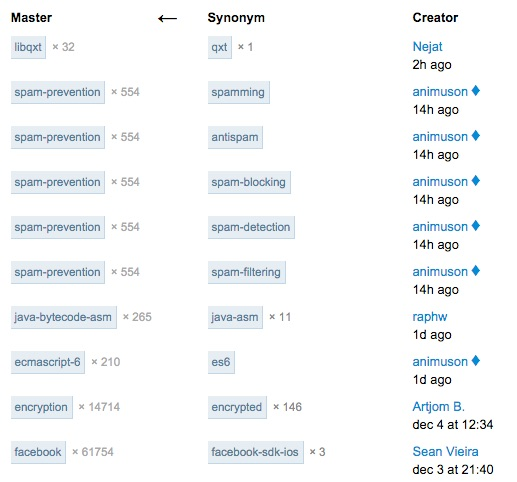
\includegraphics[width=3.2in]{tagsynonyms_so.jpg}
  \caption{Screenshot of \textit{Tag Synonyms} page.}
  \label{fig:syn}
\end{figure}

To be able to test the effects of tag synonyms on our tag recommendation model, we prepared a separate tag list derived from our initial set of $437$ after manually pruning for tag synonyms. Since these tags are among the more popular tags in the StackOverflow community, we were only able to reduce this new set to a size of $428$ after coalescing tags such as \texttt{report} and \texttt{reporting}. We expect this pruned list of tags to moderately, but not drastically, improve our results.

\subsection{Network Features}

The underlying structure of the StackOverflow network is diverse and complex since users and tags can be related through various questions, answers, and comments. We picked certain relationships between objects that we deemed to likely be the most indicative of the best tags to recommend and constructed the appropriate graphs. We briefly describe them in the following sections.

\subsubsection{Network Based on Post Similarity}

A natural graph to consider on the StackOverflow data would be the graph in which the nodes are questions and edges connect two questions if tf-idf vectors of their textual bodies have cosine similarity above a certain threshold. This graph essentially connects posts in StackOverflow based on a measure of topical similarity. The following plot shows the degree distribution of such a graph when the threshold for cosine similarity is chosen to be $0.3$.

\begin{figure}[h]
  \centering
    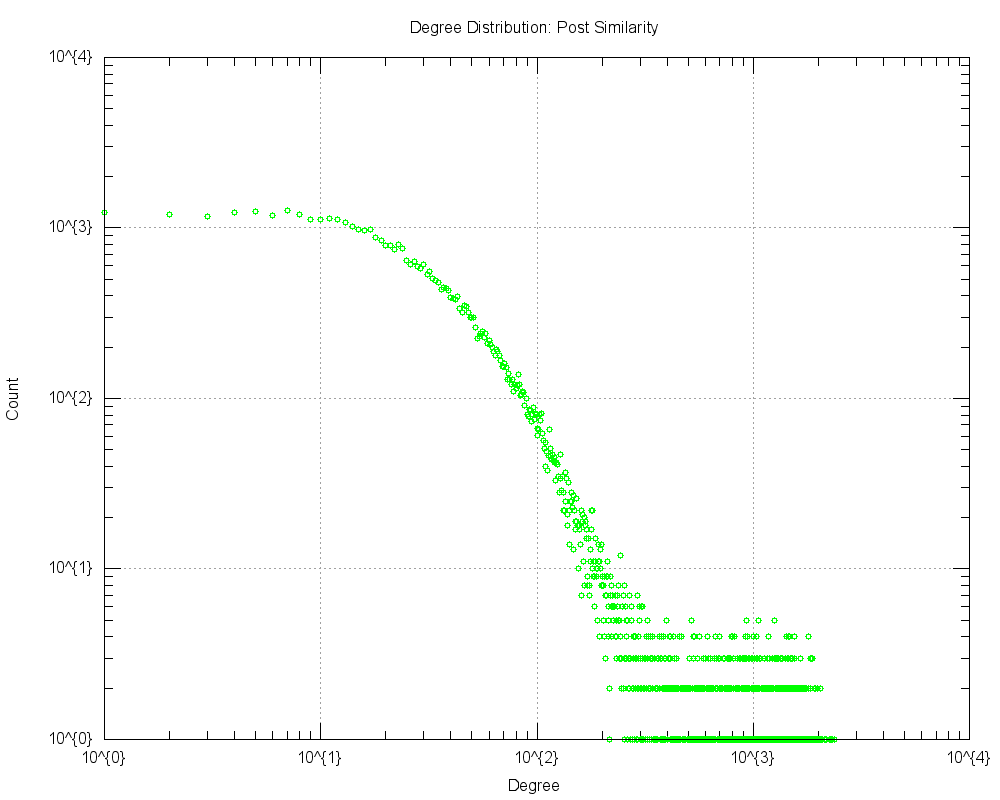
\includegraphics[width=3.2in]{similarity_degdistr.png}
  \caption{Degree distribution of the Post Similarity network.}
  \label{fig:post_dd}
\end{figure}

We notice that this degree distribution looks much like a power law distribution. Most questions are only similar to a few other questions on StackOverflow, while a few questions are similar to many others. In particular, we can observe the kinds of questions that are similar to many others. Here is one such question: http://stackoverflow.com/questions/121656/regular-expression-to-remove-xml-tags-and-their-content.
Notice that this post references XML parsing, C\#, .NET, and regular expressions, all of which are very common topics on StackOverflow. In general, the posts that have high degrees are at the intersection of multiple popular topics. This is backed up by \cite{8}, in which we see that the intersection of communities in a network are densely connected. These well-connected posts are likely to lie at the intersection of communities in this network, which motivates us to use this graph in tag recommendation. Since tags are StackOverflow’s method of organizing posts into topical categories or communities, extracting communities on this graph could lead to information about what tags to recommend to new questions that are similar to posts in a given community.

\subsubsection{Network Based on User Interaction}

We also experimented with the following StackOverflow network. The users of StackOverflow are represented as nodes of our network. Two users $u$ and $v$ are linked with an edge if $u$ answers a question posted by $v$ such that the answer reaches a predefined threshold in positive rating. In this case, two users share similar topical interests, which lead to their interactions on StackOverflow through question and answer. Below is a plot of the degree distribution of this network.

\begin{figure}[h]
  \centering
    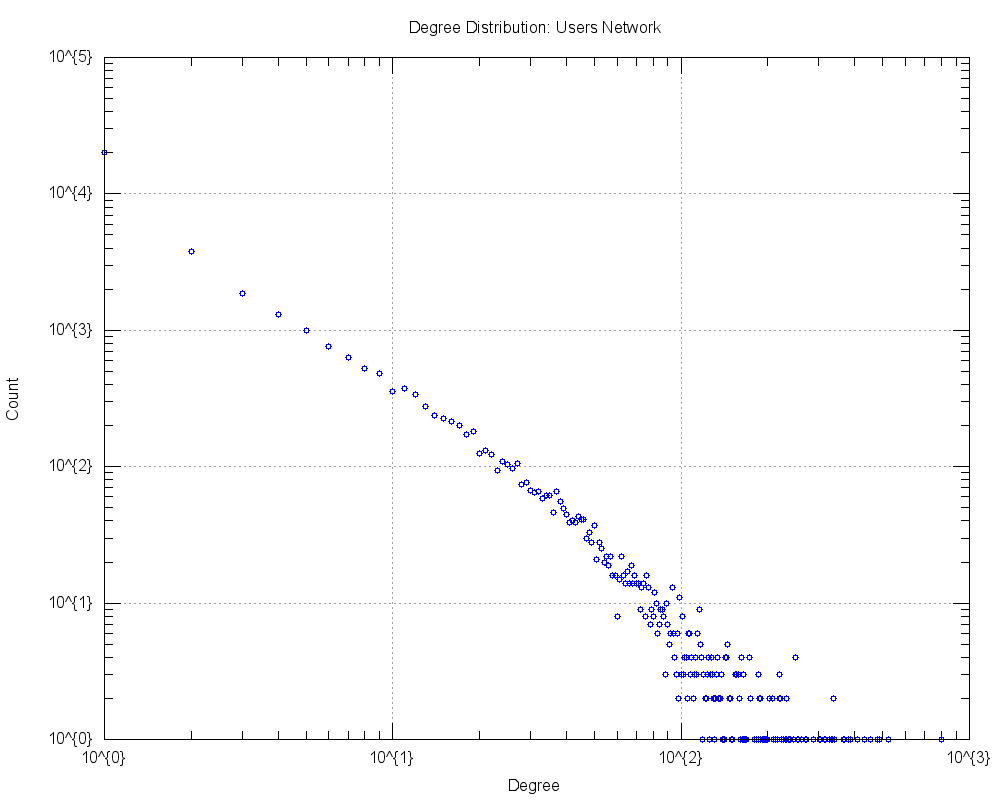
\includegraphics[width=3.2in]{user_degdistr.png}
  \caption{Degree distribution of the User Interaction network.}
  \label{fig:user_dd}
\end{figure}

The power law distribution occrus as a result of the following explanation. The users with degrees between $10$ and $100$ have the highest question to answer ratio, around $0.196$, while the users with degrees between $1$ and $10$ have the lowest question to answer ratio, around $0.118$. This means that a question posted on StackOverflow is likely to elicit multiple answers, resulting in a medium sized degree for users that post questions. Many infrequent users that answer questions will only receive interactions with the user that posted the question leading to low degrees for these users. On the extreme end, users with degree over $100$ have answered on average $148$ questions, which indicate that the tail of the distribution is populated mainly by power users or experts on StackOverflow.

The motivation for using such a graph banks on the assumption that users probably only post on a few topics in StackOverflow, and that new questions by a user are likely to share tags with a previous post. Thus, if we could organize users into communities and assign tag representatives for these communities, these tag representatives could become recommendations for questions posted by users from that community.


\subsubsection{Bipartite Graph between Users and Tags}

On sites such as Stack Overflow, relationships exist between users and tags since users will tend to interact most with the tags they are interested in or posses the most expertise with. In order to analyze these relationships we generated a bipartite graph where nodes on one side of the graph represented users and nodes on the opposite side of the graph represented tags. The edges of the graph were constructed and weighted to represent a user’s contribution and interaction with each tag. Questions, answers, and comments made by a user on a post associated with a particular tag each contributed to that user’s score with the tag in question. User made questions were evaluated as the most significant form of contribution to a tag since each post is defined by the original question and thus added the most to a user’s tag score. Answers were evaluated as the next most significant form of contribution since answers make up the majority of the structure of a post not including the question and require some level of expertise with the tags associated with the post. Comments were evaluated as significantly less indicative of a contribution to a tag since they are generally not a significant contribution to the content of a post. User tag scores were then used as weights for the edges connecting each user to each tag. Tags which scored 0 points with a user did not contain an edge to that user since this meant that the user had not interacted with the tag. Below is a plot of the degree distribution of the users in the bipartite graph.

\begin{figure}[h]
  \centering
    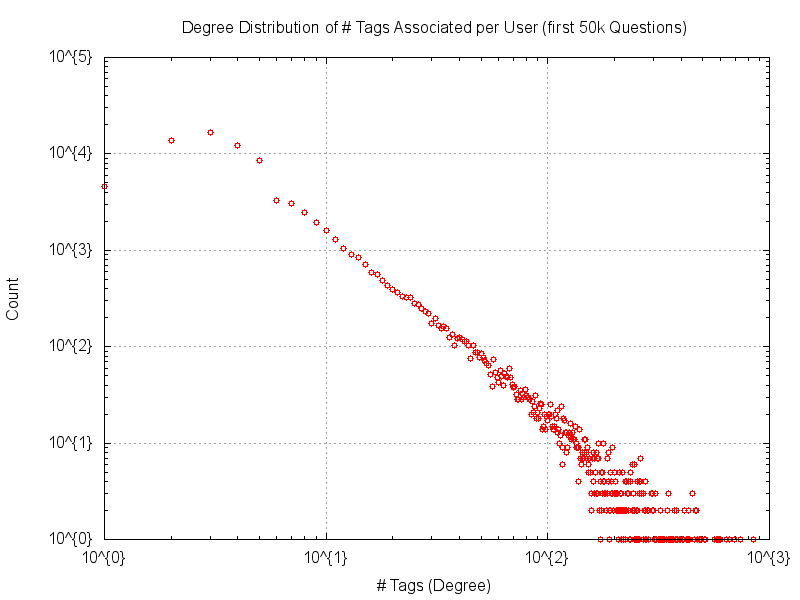
\includegraphics[width=3.2in]{bipartite_degdistr.png}
  \caption{Degree distribution of the bipartite graph between users and tags.}
  \label{fig:bi_dd}
\end{figure}

From the plot we can see that the number of tags each user was associated with followed a power law distribution. This indicates that most users interact with a very small number of tags while a select few users contribute to a large number of tags. Such a trend is consistent across many social networks with the vast majority of users having a very limited number of connections and only a small portion of users having a large amount of connections. Thus the degree distribution suggests that the users on Stack Overflow behave in a manner similar to those of other social networks. In addition, the fact that most users are associated with a limited pool of tags suggests that recommending tags based on users associated with a post could yield accurate results. For example, if the majority of users interacting on a post all have high tag scores with the same tag, then since most users have a limited pool of associated tags we can be confident that the post in question should be assigned the shared tag.

\section{Algorithm and Results}

\subsection{Original TagCombine Components}

To begin, using the procedures described in \cite{1}, we implemented the three major components of the \textit{TagCombine} algorithm to establish a baseline for the performance of our tag recommendation system. By reproducing a working implementation of \textit{TagCombine}, we were able analyze the effect of our improvements on tag recommendation accuracy.

As alluded to earlier, \cite{1} introduces the concept of the $recall@k$ metric for measuring the success of a tag recommendation model, where $k$ is a tunable parameter that determines how many tags the model recommends for each object. Intuitively, over $n$ objects, the $recall@k$ metric measures the average success rate in predicting correct tags for each object, where a ``correct'' tag is simply a tag that has been used to label that particular object by an actual user. Let $R_i$ be the set of tags recommended for object $i$ (so, $|R_i| = k$), and let $T_i$ be the actual set of tags used to label object $i$. Then, the formula for $recall@k$ is:

\[recall@k = \frac{1}{n}\sum\limits_{i=1}^{n}\frac{|R_i \cap T_i|}{|T_i|}.\]

\subsubsection{Multilabel Learning Algorithm}

The first component of \textit{TagCombine} utilizes Binary Relevance to obtain the likelihood of a post to be associated with each tag given the text of the post. Given a tag set $L$ and a question $q$, the Binary Relevance method will create $|L|$ datasets each of which corresponds to the classification of whether a different tag in $L$ should be applied to $q$ given the text in the body of $q$. Assuming that tags are independent from one another, \textit{TagCombine} performs multinomial Naive Bayes on each dataset and concatenates the resulting probabilities to obtain a score vector $Y$ whose elements $Y_i$ correspond to the probability that the $i^{th}$ tag is used to label the post. The values of the resulting score vector are then used to directly obtain the likelihood for each tag.

\subsubsection{Similarity Based Ranking Component}

The second component of \textit{TagCombine} is based on assigning tags based on similar posts. Given a new question $q$, \textit{TagCombine} first finds similar posts to $q$ using cosine similarity. First the idf of each term in our dictionary is computed. The idf of a term $t$ is given by the formula
\[ \text{idf}(t) = \frac{\# \text{ of total documents}}{\log (\# \text{ of documents containing t} )} \]
Next, for all posts $p$, the tf-idf of a term $t$ in a post $p$ is computed using
\[ \text{tfidf}(t,p) \mathbf{tf}(t, p) \times \mathbf{idf}(t)\]
where $\mathbf{tf}(t, p)$ is the raw frequency of the term $t$ in post $p$. The tf-idf vector of a post $p$, $\text{tfidf}(p)$, then refers to the vector of $\text{tfidf}(t,p)$ values over all terms $t$. The cosine similarity between an old post $p$ and the new question $q$ would therefore be
\[ \text{sim}(p, q) = \frac{\text{tfidf}(p) \times \text{tfidf}(q)}{\|p\| \|q\|}.\]
Using this cosine similarity formula, we can find $p_1, \ldots, p_{50}$, the $50$ most similar posts to $q$. Let $T_1, \ldots, T_{50}$ denote the sets of tags used in each of these posts. We compute a likelihood for each tag $g$ for question $q$ using the following formula
\[ L(g, q) = \frac{ |\{i : g \in T_i \} | }{\sum_i  |T_i |}\]


\subsubsection{Tag-term Based Ranking Component}

The third component of \textit{TagCombine} analyzes the co-occurrence of each tag with each term in order to recommend the top tags based on a post’s text. The co-occurrence, or affinity score, between a tag $t$ and word $w$ is defined as
\[ \text{co}(t, w) = \frac{\text{\# of posts with }t{ and }w}{\text{\# of posts with }t}. \]
Then, for a given post $p$ comprised of a set of words, the tag-term based ranking score for a tag $t$ is calculated as
\[ \text{TagAff}(p, t) = 1 - \prod_{w \in p}(1 - \text{co}(t, w)). \]
Intuitively, a tag $t_0$ will be recommended for a post if it shares high $\text{co}(t, w)$ affinity scores with for the words $w$ of the post. Tag $t_0$ has a high affinity score with $w$ if it had previously been used as a tag for many posts containing $w$.


\subsubsection{Analysis of TagCombine}

To establish a baseline for our tag recommendation system, we evaluated each individual component as standalone along with the entire \textit{TagCombine} algorithm itself using $10$-fold cross validation. As will be discussed more in Section 4.3, \textit{TagCombine} methodically assigns weights $\alpha$, $\beta$, and $\delta$ to the Multilabel Classifier scores, Similarity Ranking scores, and Tag Term Affinity scores respectively. Thus, the algorithm fine-tunes these parameters to determine how much (or little) each component should be applied to produce the optimal tag recommendation system. In our runs of \textit{TagCombine}, we found that $(\alpha, \beta, \gamma) = (0.6, 0.6, 0.8)$ produced the best $recall@k$ scores.

\begin{center}\begin{tabular}{c||c|c}
& $recall@5$ & $recall@10$\\ \hline\hline
Multilabel Classifier & 0.456 & 0.547\\ \hline
Similarity Ranking & 0.435 & 0.523\\ \hline
Tag Term Affinity & 0.235 & 0.326\\ \hline\hline
Our \textit{TagCombine} & 0.486 & 0.574\\ \hline\hline
\cite{1} Original \textit{TagCombine} & 0.596 & 0.724\\
\end{tabular}\end{center}

We can see that our standard implementation of \textit{TagCombine} does significantly worse than the cited \textit{TagCombine}. To remedy for this, we also calculated tag-adjusted $recall@k$ scores. From earlier, we defined $T_i$ to be the set of all tags that are actually used to label post $i$. The description of $recall@k$ in \cite{1} is ambiguous in explaining whether an element of $T_i$ can be any tag in the StackOverflow network, as we assumed in the first table, or only the top $437$ that we filtered in Section 3.1. So, we define $recallAdj@k$ scores to be calculated the same as $recall@k$ except that $T_i$ can contain tags only from the list of the top $437$.

\begin{center}\begin{tabular}{c||c|c}
& $recallAdj@5$ & $recallAdj@10$\\ \hline\hline
Multilabel Classifier & 0.587 & 0.703\\ \hline
Similarity Ranking & 0.569 & 0.681\\ \hline
Tag Term Affinity & 0.304 & 0.420\\ \hline\hline
Our \textit{TagCombine} & 0.617 & 0.748\\ \hline\hline
\cite{1} Original \textit{TagCombine} & 0.596 & 0.724\\
\end{tabular}\end{center}

Our $recallAdj@k$ scores are much closer to those from the original \textit{TagCombine} algorithm. However, as a reminder, we are only interested in how applying the underlying StackOverflow network can potentially improve upon our tag recommendation model, and so the interesting results will be the difference between the $recall@k$ (or $recallAdj@k$) scores of our new model and those of our baseline. Our method of calculating scores and the actual score values do not matter as long as they are consistent.

Clearly, the composite \textit{TagCombine} score is not a linear combination of its individual components. So, before continuing on to improve \textit{TagCombine}, we also analyzed the contribution of each individual component to the \textit{TagCombine} scores, using $recall@5$ as an example. To do so, we held two parameters constant at their optimal values while varying the third. The Multilabel Classifier is weighted by $\alpha$, Similarity Ranking is weighted by $\beta$, and Tag Affinity is weighted by $\gamma$, so to test the significance of the Similarity Ranking component, for example, we held $\alpha$ and $\gamma$ constant while varying $\beta$. Figure~\ref{fig:tc_alpha}, Figure~\ref{fig:tc_beta}, and Figure~\ref{fig:tc_gamma} plot $\alpha$, $\beta$, and $\gamma$, respectively.

\begin{figure}[h]
  \centering
    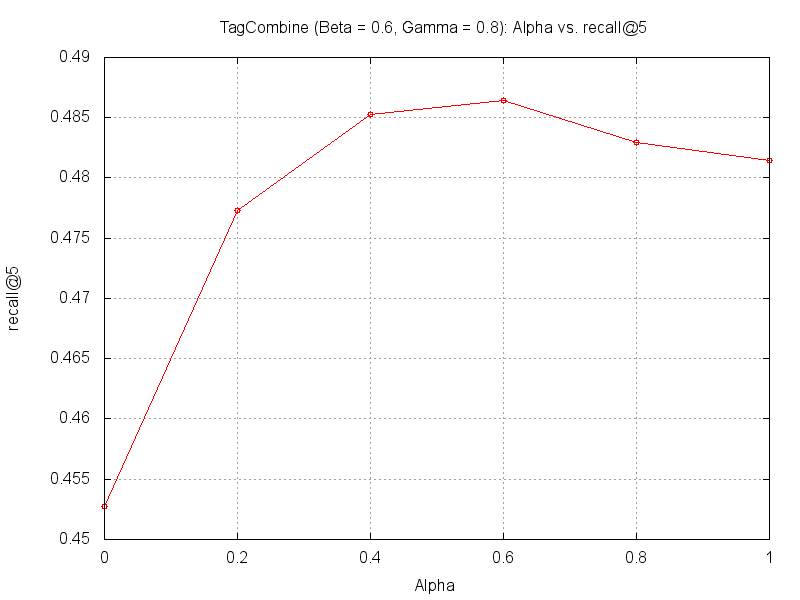
\includegraphics[width=3.2in]{tc_alpha.png}
  \caption{Multilabel Classifier contribution to \textit{TagCombine}.}
  \label{fig:tc_alpha}
\end{figure}

\begin{figure}[h]
  \centering
    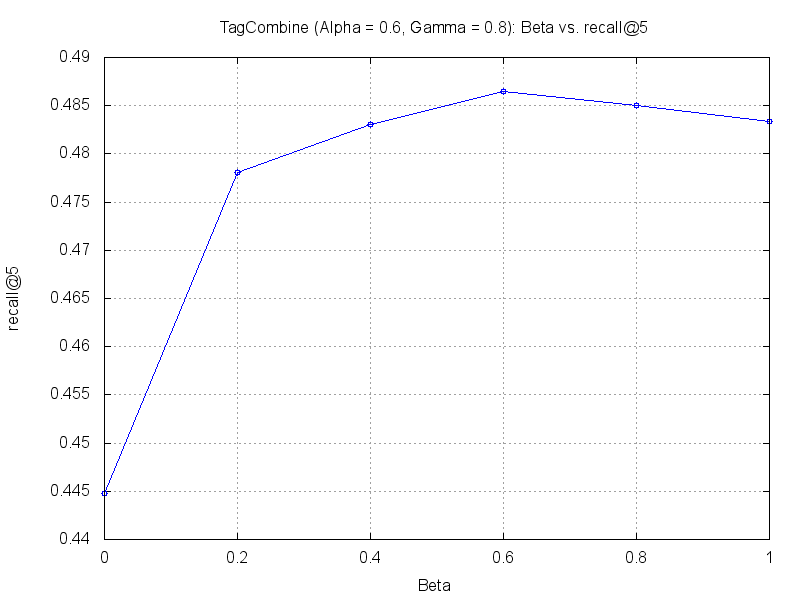
\includegraphics[width=3.2in]{tc_beta.png}
  \caption{Similarity Ranking contribution to \textit{TagCombine}.}
  \label{fig:tc_beta}
\end{figure}

\begin{figure}[h]
  \centering
    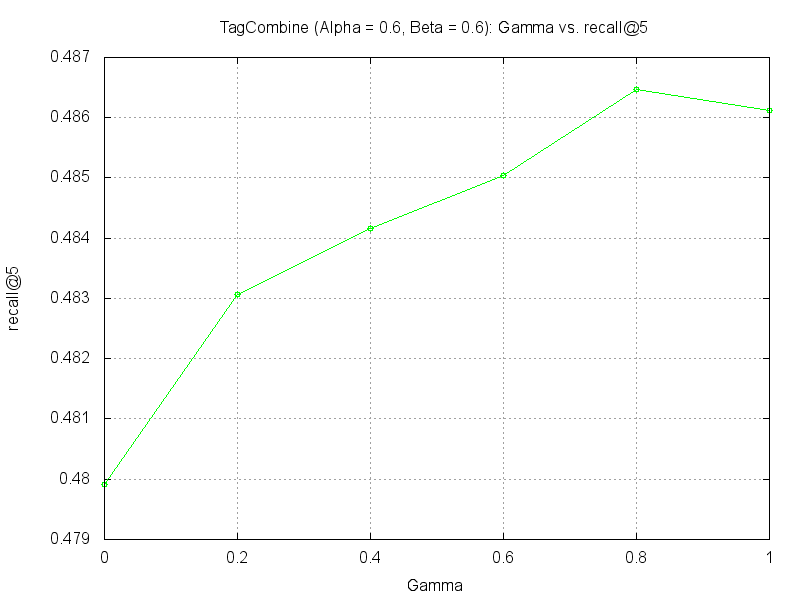
\includegraphics[width=3.2in]{tc_gamma.png}
  \caption{Tag Affinity contribution to \textit{TagCombine}.}
  \label{fig:tc_gamma}
\end{figure}

One way we can measure the contribution of each individual component is to compare the $recall@5$ score when its corresponding parameter’s value is $0$ (not used) and to when the value is optimal. We can see that the Similarity Ranking component has the most significant contribution ($\approx 0.041$), then the Multilabel Classifier component ($\approx 0.03$), and finally the Tag Affinity component ($\approx 0.006$). So, when evaluating the improvements in our new tag recommendation model, in addition to comparing composite $recall@k$ scores, we can also look at the contribution of our added network component.


\subsection{Network Based Improvements to TagCombine}

In order to improve upon the tag recommendation accuracy of \textit{TagCombine} we sought to include components that utilized the structure of networks present in the Stack Overflow data. Preliminary analysis of the graphs in section 3 supported our original intuition that user and tag interactions on Stack Overflow did exhibit behavior consistent with the interactions of users on more classical examples of social network sites. By leveraging this behavior we constructed components that could accurately recommend tags using the structure present in the underlying networks of Stack Overflow and without relying on textual data. Incorporating these improvements into \textit{TagCombine} would allow us to add another dimension of information to the original algorithm and obtain results that leverage more of the data present in Stack Overflow.

\subsubsection{New Component}

Our primary improvement to \textit{TagCombine} was the addition of a fourth component that utilized the network structure stemming from the interaction of users with tags to predict the probability of each tag being associated with a given post. We begin by constructing the bipartite graph between users and tags described in section 3.3.3. Given a post $p$, we compile a list of users who contributed to $q$ and use the edge weights between the users and each tag to determine the tag’s ranking score. Define $Q_i$ to be the edge weight between the user who posted the original question of $p$ and the $i^{th}$ tag and $B_i$ to be the edge weight between the user who posted the best answer for $p$ and the $i^{th}$ tag. Next ,for each comment in $p$ sum up the edge weights between the user who posted the comment and the $i^{th}$ tag, define this value to be $C_i$. Now for each answer in $p$ find the sum of the edge weights between the user who posted the answer and the $i^{th}$ tag and let this value be $A_i$. Using these values, the score for the $i^{th}$ for post $p$, $S_i$ is given by:
\[ S_i = \alpha Q_i + \beta B_i + \gamma C_i + \delta A_i \]
where $\alpha$, $\beta$, $\gamma$, and $\delta$ are constant weights evaluated by 10-fold cross validation to maximize tag recommendation accuracy. Calculating the score value $S_i$ for each tag gives us the likelihood of each tag to be used to label $p$.

\subsubsection{Modification to Similarity Component}

The second improvement we made to TagCombine was to add features based on community detection to the similarity component. Using the graph in 3.3.1, we first run the SNAP implementation of BigCLAM to group posts in StackOverflow into 1000 different communities, which we will label $C_1 , \ldots, C_{1000}$. For each community $C_j$, define the set of tag representatives $R_j$ to be the set of tags that appear in at least $80\%$ of the posts in $C_j$. In the similarity component of \textit{TagCombine}, we now make the following modifications to the computation of the likelihood of assigning a tag $g$ to a new question $q$.
\[ L(g, q) = \frac{ |\{i : g \in T_i \}| + \sum_i |\{j : p_i \in C_j \text{ and } g \in R_j \}| }{\sum_i  |T_i | + \sum_i |\{j : p_i \in C_j\} |} \]
That is, of the top $50$ similar posts $p_1, \ldots, p_{50}$, each community these posts belong in will also be able to contribute their tag representatives to the likelihoods of assigning tags to the new question $q$.


\subsection{NetTagCombine Algorithm}

In our proposed tag recommendation system, \textit{NetTagCombine}, we add our new Network-Based Ranking Component, alongside the other components of \textit{TagCombine}. Building upon the equation for \textit{TagCombine} given in \cite{1}, for all tags $t$ with respect to some post $p$, our new \textit{NetTagCombine} score can be given by
\begin{align*}
NetTagCombine_p(t) =\ &\alpha \times MultiLabel_p(t) +\\
&\beta \times SimRank_p(t) +\\
&\gamma \times TagTerm_p(t) +\\
&\delta \times Network_p(t)
\end{align*}
where $\alpha,\beta,\gamma,\delta \in [0,1]$ represent the different weights of the components. Here, we have added the term of $\delta \times Network_p(t)$ to represent our new fourth component that uses the underlying network structure. To adjust for this fourth component, here is the pseudocode for \textit{NetTagCombine}:


\begin{algorithm*}
  \caption{\textit{NetTagCombine} algorithm}\label{ntc}
  \begin{algorithmic}[1]
    \State $\alpha, \beta, \gamma, \delta \gets 0$
    \For{\textbf{all }posts $p$}
      \For{\textbf{all }tags $t \in TAGS$}
        \State Compute \textit{MultiLabel}$_p(t)$, \textit{SimRank}$_p(t)$, \textit{TagTerm}$_p(t)$, and \textit{Network$_p(t)$}
      \EndFor
    \EndFor
    \For{\textbf{all }$\alpha$ from $0$ to $1$, every time increment by $0.2$}
      \For{\textbf{all }$\beta$ from $0$ to $1$, every time increment by $0.2$}
        \For{\textbf{all }$\gamma$ from $0$ to $1$, every time increment by $0.2$}
          \For{\textbf{all }$\delta$ from $0$ to $1$, every time increment by $0.2$}
            \State Compute \textit{NetTagCombine}$_p(t)$ for all tags $t$ on posts $p$
            \State Evaluate effectiveness of $(\alpha,\beta,\gamma,\delta)$ from $recall@k$ scores
          \EndFor
        \EndFor
      \EndFor
    \EndFor\\
    \Return Best $(\alpha,\beta,\gamma,\delta)$\;
  \end{algorithmic}
\end{algorithm*}

\subsection{Results of NetTagCombine}

\subsection{Other Considerations}

We also tried to use BigCLAM to detect user communities on the graph in section 3.3.2. For each user community $U_i$, we would compute the set of tag representatives $S_i$ for $U_i$. A tag $g$ would be in in $S_i$ if at least $80\%$ of the users in the community have posted a question or answered a question that was tagged with $g$. Then given a question posted by an existing user $u$, we would loop through all $U_i$ the user belonged in and compute a likelihood for assigning a tag $g$ to the user as
\[ L(g, u) = \frac{|\{i : g \in S_i\} |}{\sum_i |S_i|}. \]
That is, the likelihood of assigning tag $g$ to a question posted by user $u$ would be proportional to the frequency the tag appeared as a representative of the communities $u$ was in. However, adding this component did not improve the performance of NetTagCombine, as it is likely that any information produced by this network component is redundant with those outputted by our improvements in sections 4.2.1 and 4.2.2.

\section{Conclusion}

Something about how we did better.

It should be noted that, although \textit{EnTagRec} produced better results, we chose to use \textit{TagCombine} as a baseline for measuring our improvements to tag recommendation. There were several reasons for this decision. First, \textit{TagCombine} uses a generally simpler algorithm which made it easier to accurately reproduce. In addition, \textit{EnTagRec} incorporates some degree of network structure while assessing the accuracy of its tag recommendations. Thus, using \textit{TagCombine} as a baseline allows us to more clearly demonstrate the improvement caused by incorporating network structure. Finally, we used different and more complex network analysis methods from the simple ones implemented in \textit{EnTagRec}, so it is likely that our improvements would cause a similar increase on the $recall@k$ scores of \textit{EnTagRec}.

\subsection{Future Work}

As discussed in Section 2.3, we chose to evaluate our network-based improvements upon an implementation of \textit{TagCombine} instead of the more recent \textit{EnTagRec}. Future work, then, could apply our improvements to an implementation of \textit{EnTagRec} and analyze whether \textit{EnTagRec} improves in a similar manner to what we have in \textit{TagCombine}. Furthermore, incorporating a network component into our model invites the possibility of a dynamic tag recommendation system. Tagging a post is not an action limited to post creation time. While this has already been addressed simply by the fact that we are using user interaction and collaboration -- events that happen after post creation -- to assist tag recommendations, we have so far only modeled the network based on one snapshot in time. Since we have access to the entire log of post edit history, it would be interesting to see how our tag recommendations and $recall@k$ scores would change over time given snapshots in which more or less users had contributed to certain posts. Any discovered insights or trends would provide commentary on the effectiveness of future dynamic tag recommendations systems that constantly restructure their models along with the network itself.


\begin{thebibliography}{1}
\bibitem{1} X. Xia, D. Lo, X. Wang, B. Zhou. Tag Recommendation in Software Information Sites. MSR, 2013.
\bibitem{2} S. Wang, D. Lo, B. Vasilescu, A. Serebrenik. EnTagRec: An Enhanced Tag Recommendation System for Software Information Sites. ICSME, 2014.
\bibitem{3} J. McAuley, J. Leskovec. Discovering Social Circles In Ego Networks. ACM TKDD, 2014.
\bibitem{4} M. Girvan, M. E. J. Newman. Community Structure in Social and Biological Networks. National Academy of Sciences, 2002.
\bibitem{5} A. Clauset, M. E. J. Newman, C. Moore. Finding Community Structure in Very Large Networks. APS, 2004.
\bibitem{6} G. Palla, I. Der\'{e}nyi, I. Farkas, T. Vicsek. Uncovering the Overlapping Community Structure of Complex Networks in Nature and Society. Nature, 2005.
\bibitem{7} J. Yang, J. Leskovec. Overlapping Community Detection at Scale: A Nonnegative Matrix Factorization Approach. WSDM, 2013.
\bibitem{8} J. Yang, J. Leskovec. Community-Affiliation Graph Model for Overlapping Network Community Detection. ICDM, 2012.
\bibitem{9} Stack Exchange Data Dump (September 26, 2014). Retrieved 2 November 2014. https://archive.org/details/stackexchange.

\end{thebibliography}

\appendix

Individual contributions of group members:
Logan: worked on code for TagCombine, worked on code for NetTagCombine, wrote final paper
Chris: worked on code for TagCombine, worked on code for NetTagCombine, wrote final paper
David: worked on code for TagCombine, worked on code for NetTagCombine, wrote final paper
We feel that each member did an equal and fair amount of work, and we request that we each be given the same individual grade.


%\balancecolumns

\end{document}
